\chapter{Class Diagrams and Interface Specifications}

\section{Class Diagram}
\begin{figure}[h]
\centering
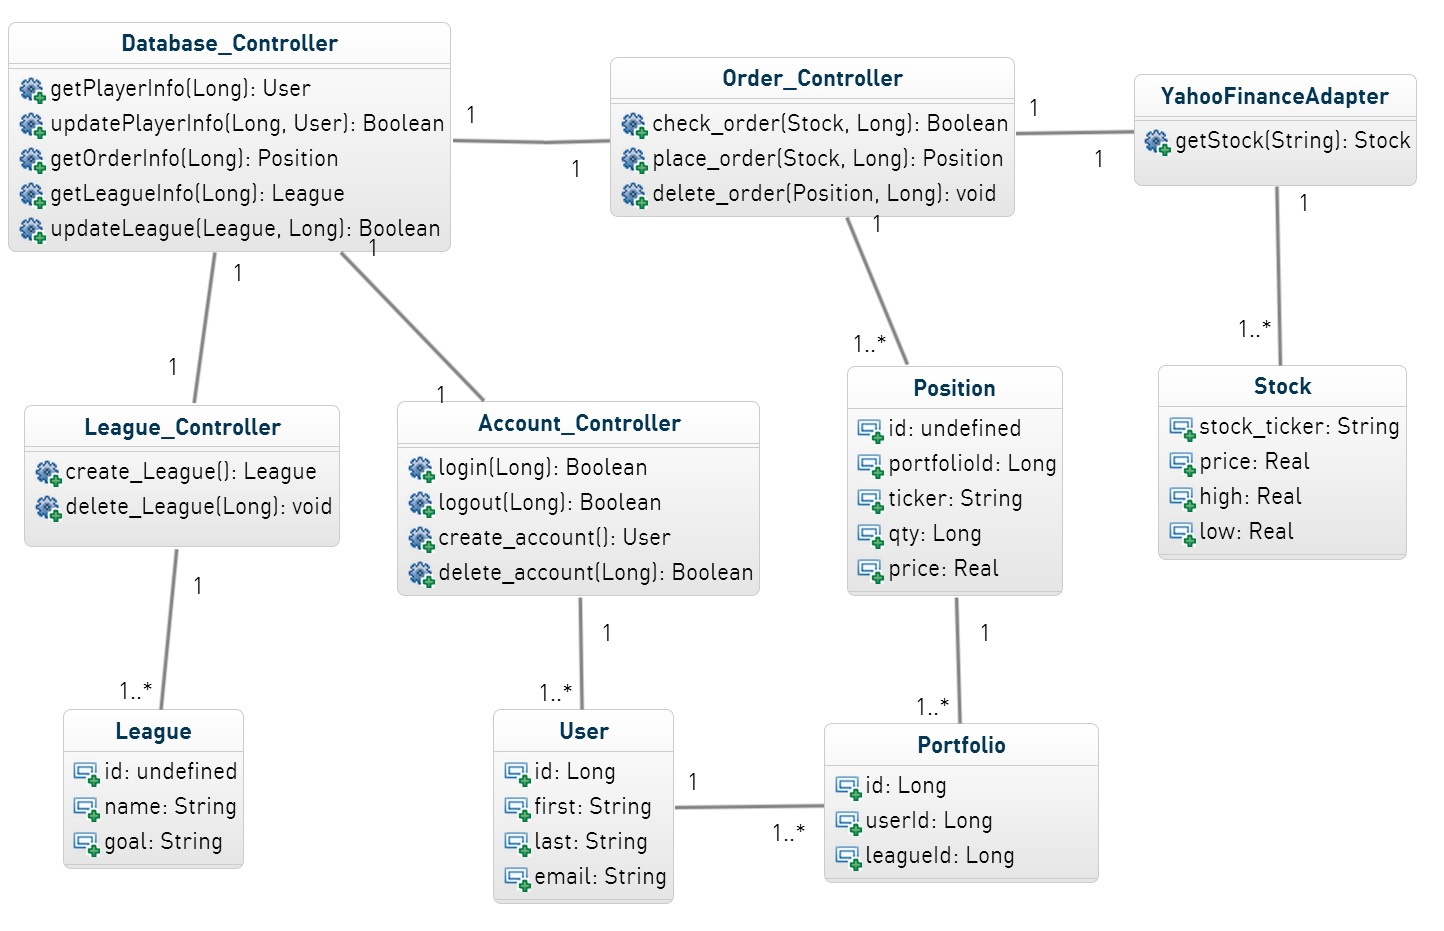
\includegraphics[width=5.5in]{./img/classDiagram.jpg}
\end{figure}


\clearpage

\section{Class Data Types and Operation Signatures}

\subsection{Database Manager}
Our database manager performs the function of managing the database. This can
mean anything from adding user information into the database, retrieving
information from the database and updating information in the database,
regardless of whether the information deals with users/accounts, leagues,
orders. \\*

{\bfseries Methods} \\*

{\bfseries + get_player_info(in user_id : long) : class User } \\*
	This method is used when information needs to be retrieved for a specifc
  player \\*

{\bfseries + update_player_info(in user_id : int, in upd: class user) : bool } \\*
    This method is used to update a user’s information, whether it be
    administrative or game related. \\*

{\bfseries + get_order_info(in transaction_id : int) : class transaction } \\*
	This method takes in a transaction id and returns the information associated
  with that specific transaction.\\*

{\bfseries + update_league(in league_id : int, in leagueInfo : class league) : bool } \\*
	This method returns the latest updates in the league \\*

{\bfseries + return_league_updates(in league_id : int) : class league  }\\*
This method is used when a league needs to be updated with the newest
information provided in the league in the input
	 \\*

\subsection{Order Manager}


Our order manager class is responsible for handling all the tasks related to
orders/transactions. It is responsible for placing the order in the system and
for moving old orders to the archive transactions table.
 \\* \\*

{\bfseries Methods} \\*

{\bfseries + Check_order(in symbols: class Order) : bool} \\*
This method is simple used to check and make sure that the input order can be
processed. It will check the users balance, etc.
     \\*

{\bfseries + place_order(in symbols: class Order) : bool } \\*
As the name suggests, this method is used to place an order in the system, with
the information given by the input Stock class.
	\\*

{\bfseries + delete_order(in symbols: transaction_id): bool } \\*
	As the name suggests, this method deletes an order from the system, assuming
  that it hasn’t already been processed. If it has then this function will
  return a false value.\\*

{\bfseries + Execute_order(in transaction_id : int) : bool } \\*
	This method is responsible for actually getting the stock
    information from Yahoo Finance API and then changing the
    account/portfolios to reflect it accordingly. \\*

\subsection{League Manager}

This class is responsible for managing all the leagues in the system. It has
the authority to create leagues, delete leagues, and modify leagues as it is
instruction to do so. \\* \\*

{\bfseries Methods} \\*

{\bfseries + Create_league () : Class league } \\*
	This function is used to create a league from scratch so that the user can
  create a league. \\*

{\bfseries + Delete_leagues(in league_id : int) : bool } \\*
	As the name suggests, this method will delete the league matching the input\\*

{\bfseries + change_league_name( in league_id : int) : bool } \\*
	This method is here solely for the purpose implied by its
    name.  It’s only function is to change the name of the
    league.  \\*

{\bfseries + Change_league_manager (in league_id : int, in usr : class User) : bool } \\*
	This function replaces the current league manager stored
    in the input league with the user specified in the input. \\*

{\bfseries + add_rules(in league_id : int) : bool } \\*
	This function is here for the reason its name suggests.
    It is here just to add rules to a given league.  \\*

{\bfseries + Delete_rules(in league_id : int) : bool } \\*
	This method exists just to delete the rules in a league.  \\*


\subsection{Account_Controller}
This class exists to take care of any function that relates to accounts. This
can mean creating an account, modifying an account, or even deleting
 \\* \\*

{\bfseries Methods} \\* \\*

{\bfseries + Login(in user_id : int) : bool} \\*
	This function is used by the user to log into the system

{\bfseries + logout(in user_id : int) : bool } \\*
	This function is the opposite to the one above it, it is
    used by the User to log out of the system. \\*

{\bfseries + Verify_User(in User_id : int) : bool} \\*
	Method to make sure that the person logging in or that
    the person who is logged in is not an imposter/fake. \\*

{\bfseries + Create_account() : class User } \\*
	Creates an account with the current user  \\*

{\bfseries + delete_account(in suser_id : int) : bool } \\*
	Used to delete an account from the database system.   \\*

\subsection{Yahoo Finanace Adapter}
This class is responsible for obtaining market data from Yahoo Finance
API.  It consists of 3 functions to get quotes, get company information,
and to get sector information.

{\bfseries Methods} \\* \\*

{\bfseries + Get_quote(in stock_ticker_id : string) : class quote } \\*
	As the name suggests, this method is responsible for obtaining
    quote information about a given stock_ticker \\*

{\bfseries + get_company_info(in stock_ticker_id : string) : class Company } \\*
	This method is responsible for getting market information about a
    specified company.  \\*

\subsection{Stock}
This class is responsible for representing a Stock. It has the authority to hold
a ticker symbol, price, daily high price, and daily low price. \\* \\*

{\bfseries Attributes} \\*

{\bfseries + String:stock_ticker} \\*
This attribute holds the ticker symbol as a character array.\\*
{\bfseries + double:price} \\*
This attribute holds the current value of stock corresponding to the ticker
symbol.\\*
{\bfseries + double:high} \\*
This attribute holds the current High price of the stock on the market.\\*
{\bfseries + double:low} \\*
This attribute holds the current Low price of the stock on the market.\\*

\subsection{User}
This class is responsible for representing a User. It has the authority to hold
first name, last name, email address, and userId.\\* \\*

{\bfseries Attributes} \\*

{\bfseries + long:id} \\*
A unique id to distinguish different users from one another. \\*
{\bfseries + String:first} \\*
This attribute holds the first name of the user. \\*
{\bfseries + String:last} \\*
This attribute holds the last name of the user. \\*
{\bfseries + double:low} \\*
This attribute holds the email address of the user. \\*


\subsection{Position}
This class is responsible for representing a Position, which is a stock that a
user owns. It has the authority to hold the user Id, portfolio Id, ticker
symbol, quantity and price.\\* \\*

{\bfseries Attributes} \\*

{\bfseries + long:id} \\*
A unique id to distinguish different users from one another. \\*
{\bfseries + long:portfolioId} \\*
A unique id to distinguish different users from one another. \\*
{\bfseries + String:ticker} \\*
This attribute holds the first name of the user. \\*
{\bfseries + long:qty} \\*
This attribute holds the quantity of the certain position.\\*
{\bfseries + double:price} \\*
This attribute holds the price that the position was purchased at.\\*

\subsection{Portfolio}
This class is responsible for representing a Portfolio, which is the set of
stocks that a user owns. It has the authority to hold the user Id, portfolio
Id, ticker symbol, quantity and price. \\* \\*

{\bfseries Attributes} \\*

{\bfseries + long:id} \\*
A unique ID to distinguish different portfolios from one another.\\*
{\bfseries + long:userId} \\*
A unique ID to distinguish who owns the portfolio. \\*
{\bfseries + String:leagueId} \\*
A unique ID to distinguish what league this portfolio is a part of. \\*

\subsection{League}
This class is responsible for representing a League, which is a group that
users can belong to, to compete with each other.\\* \\*

{\bfseries Attributes} \\*

{\bfseries + long:id} \\*
A unique ID to distinguish different portfolios from one another.\\*
{\bfseries + String:name} \\*
This attribute holds the name of the league.\\*
{\bfseries + String:goal} \\*
This attribute holds the necessary requirement for a person to be declared the
winner of a league. \\*



\iffalse


\subsection{Object Constraint Language}
In order to separate ideas in OCL, we will split it up descriptions by each class in the class diagram.
\subsubsection{Finanace Adaptor Class}
In this class, we have a few constraints that deal with this class being kind of central to all of the other classes that make up our financial adaptor. The function to buy or sell stocks are the same in their constraints. You must have a symbol name which is not equivalent to NULL and is the symbol of a company that exists. The amount must be a positive integer and if you are buying you must have enough to spend on this. Lastly, the userID must be plugged in, so that must also not be NULL and it should hold the username of someone who exists. The function get\_company\_data must have a symbol passed in that exists and is not NULL. The function scan\_list must be called after the list already exists, or there will be an error. Lastly, the update\_companies function must have a return from EoDdata that is valid and not corrupted.
\subsubsection{Current Companies}
All three of the functions in this class have the same constraint, that the symbol passed in must exist. On top of that, the ``length'' variable must always be equal to the amount of symbols in the ``symbols'' variable.
\subsubsection{Yahoo! Finanace Class}
Fortunately for us, this is another simple addition for it is dealt with completely by Yahoo! Finance. Something that we do have to be careful of is making sure that if we are calling the get\_quotes or get\_hist\_quotes, we have to make sure that we are passing in a valid string. For example, if we passed in a NULL string, we would have an error returned.
\subsubsection{EoDdata Class}
This is the simplest class out of any of the ones we deal with, as there are no variables and only one function that returns a large list of stocks without us having to pass in anything. No constraints in this class.
\subsubsection{Sector and Quote Class}
The constraints on these classes will work as long as Yahoo! Finanace returned results that are valid. These results are checked in the Finance Adaptor Class, and if it did make it past that point, the data that is passed in is fine, and therefore there are no actual constraints on these classes.


\section{Design Patterns}
Various standard design patterns were utilized to provide functionality for things such as authentication, efficient page rendering and object modeling.
\subsection{Model-View-Controller}
The Model-View-Controller (MVC) pattern was heavily used throughout the CapitalGames system to properly organize model logic, business logic and presentation logic. This very intuitive pattern allowed the team to easily delegate work on different levels of the system. Frequently, a selection of team members would develop front-end functionality which required only the views to be altered, while other members implemented backend functionality which was done either in controllers or models. This pattern resulted in a more efficient development lifecycle overall, while also providing some performance gains. Namely, the MVC pattern calls on resources only when they are actually needed which prevents unnecessary overhead. For example, methods developed to be called only programmatically don't attempt to display a view which results in faster responses.
\subsection{Security Proxy}
The security proxy pattern was the core of our secure authentication system. This proxy pattern allowed us to easily protect content based on user role or other variables. The security proxy was implemented very similarly to that described in the textbook. Particularly, it behaved as a transparent filter between an HTTP request and a controllers method. Authentication requirements could easily be chained onto each other making it possible to create custom controller prerequisites. Finally, because the security proxy filtered every request made on a controller instead of just requests made upon login, all sensitive features of the site had a very robust shell which no user could easily bypass. This improved our design by providing solid, system-wide security.
\subsection{ActiveRecord Pattern}
The ActiveRecord pattern, an intelligent implementation of a database access design pattern, was used exclusively to interact with persistant storage technologies used in the CapitalGames system. This pattern offered the major advantage of not needing to hard code any database-specific queries. All requests made to the ActiveRecord Pattern are translated to the currently used DB system's language and data is returned in directly its object form. The lack of need to write direct queries also lead to a great side effect, namely database agnosticism which allowed various database implementations to be used during different stages of development. During developmnt SQLite was used for its lightweight footprint on the developers machine, then for production MySQL was used as it is considerably more efficient when dealing with larger amounts of data. This design certainly improved our development by saving countless hours of development time.
\subsection{RESTful Design}
The RESTful design pattern being used more and more now on the web allowed us to implement our asynchronous order processing system. The RESTful design of some internal functionality allowed it to be accessed programmatically and securily through a simple API. As RESTful services are at the heart of Ruby on Rails, it did not require a lot of effort to expose some internal functionality without creating major security holes. Future iterations of CapitalGames will continue to rely on the stateful communication that our RESTful API offers.
\subsection{Responsive UI Pattern}
The Bootstrap UI framework implemented a design pattern completely segregating visual presntation from content and user experience. This provided in a beautiful responsive design which adapted to different client devices ranging from desktops to smartphones. The pattern takes advantage of the flexible markup of HTML5 to customize it on the fly when the page is rendering in the browser using Javascript and CSS. This allowed our team to target the rapidly growing mobile users without much extra implemetation effort. It also inherently produced a faster user experience since minimal processing is done during initial page rendering and mostly done asynchronously once the page is already viewable to the user. We actively strived to achieve both of these goals.
\fi
